\chapter{Continuous State Space Models with Count Observations}
\label{chap:eight}

The past two chapters have explored different notions of latent
state: a dynamic network in Chapter~\ref{chap:six} and a discrete
latent state in Chapter~\ref{chap:seven}. These notions are a powerful
addition to the autoregressive models of the earlier chapters. In
this chapter, we consider one final extension --- a continuous
latent state that evolves over time. These continuous latent state
space models are one of the most common methods in computational
neuroscience \citep{Smith-2003, paninski2010new, macke2011empirical,
  Buesing12, Petreska-2011, cunningham2014dimensionality}.

In general, these methods typically assume that the latent state obeys
linear dynamics. Here, however, we will consider the more general case
in which the dynamics are only \emph{conditionally} linear given a
dynamic discrete latent state \citep{Petreska-2011}.  This is known as
a \emph{switching} linear dynamical system.  By switching between
different linear dynamical regimes, we obtain highly nonlinear
patterns of dynamics. Moreover, this switching linear dynamical system
will recover a number of common models as special cases.

The challenge, as should be expected by now, is in performing
efficient inference in the face of discrete observations. The
aforementioned existing methods have relied upon a Laplace
approximation to the Poisson likelihood, which are asymptotically
biased. Given the tools developed in previous chapters, we can now
develop asymptotically exact Gibbs sampling algorithms. In particular,
the \polyagamma augmentations introduced in Chapter~\ref{chap:five}
will make it easy to develop efficient algorithms that leverage many
of the standard tools that exist for Gaussian observation models. Once
we have augmented our observations with \polyagamma auxiliary
variables, they appear as Gaussian observations to the latent
states. Thus, all of our tools for efficient Bayesian inference in
linear Gaussian models are at our disposal.
%In particular, we will
%derive a block Gibbs sampling algorithm and show that it outperforms
%alternative approaches based on Laplace approximations to the
%nonconjugate Poisson likelihood.

Finally, we will consider a problem that we have given little
consideration thus far, namely, the problem of Bayesian model
comparison.  We have tacitly assumed that predictive likelihoods
provide a sufficient means of comparing two models. In practice, this
has led to some difficulty, as we encountered with the network model
comparison in Chapter~\ref{chap:five}. The root cause is that
predictive likelihood comparisons only implicitly depend on model
complexity by relying on overfitting to implement a form of Occam's
razor.  In theory, the marginal likelihood --- the denominator in
Bayes' rule --- should provide a better estimate of the trade-off
between how well a model fits the data and the size of the hypothesis
class.

We will show how the fully-conjugate models derived via \polyagamma
augmentation enable principled marginal likelihood estimation
via annealed importance sampling (AIS) \citep{neal2001annealed}. In order
to make this practically feasible, however, we must dive into the
guts of the \polyagamma distribution and develop a novel sampling
algorithm capable of efficiently generating random variates in the
``small shape'' regime required by AIS. 
 
 
\section{Continuous Latent State Space Models}
Consider a general formulation of models with a continuous latent
state,~$\bx_t \in \reals^D$, with affine, but potentially nonstationary,
dynamics at time~$t$ governed by~$\bA_t$,~$\bb_t$, and
covariance,~$\bSigma_t$. Let the initial state distribution have 
mean~$\bmu_1$. Furthermore, assume that a linear activation model
~$\bpsi_t = \bC \bx_t$, where the mean spike count,~$s_{t,n}$ is 
a nonlinear function of~$\psi_{t,n}$ and neuron-specific parameters,~$\nu_n$.
We refer to the collection of model parameters as,
\begin{align*}
  \btheta = \left\{ \{\bA_t, \bb_t, \bSigma_t\}_{t=1}^T, \bmu_1, \bC, \{\nu_n\}_{n=1}^N \right\}
\end{align*}
Given these parameters, we can summarize this probabilistic model.  In
keeping with standard texts \citep[e.g.][Chapter
18]{murphy2012probabilistic}, we use ``Matlab'' notation to refer to
a sequence of spike count vectors,~$\bs_{1:T}$, and a sequence of
latent state vectors,~$\bx_{1:T}$. We have,
\begin{align*}
  p(\bs_{1:T}, \bx_{1:T} \given  \btheta) 
  &= 
    p(\btheta) \, p (\bx \given \btheta) \, p(\bs_{1:T} \given \bx_{1:T}, \btheta)
\end{align*}
where
\begin{align}
  \nonumber
  p(\bx_{1:T} \given \btheta) 
  &= 
    \distNormal(\bx_1 \given \bmu_1, \bSigma_1) \,
    \prod_{t=2}^T \distNormal(\bx_t \given \bA_t \bx_{t-1} + \bb_t, \bSigma_t)
  \\
  \nonumber
  p(\bs_{1:T} \given \bx_{1:T}, \btheta) 
  &= 
    \prod_{t=1}^T p(\bs_{t} \given \bC \bx_t, \{\nu_n\}) \\
  \label{eq:s_likelihood}
  &=
    \prod_{t=1}^T \prod_{n=1}^N p(s_{t,n} \given \psi_{t,n}, \nu_n).
\end{align}

Now consider the special case where there are only~$K$ unique dynamics
and covariance matrices,~${\{\bA_k, \bb_k, \bSigma_k\}_{k=1}^K}$, and that at
any instant in time, the chosen dynamics are specified by the
discrete latent variable~${z_t \in \{1, \ldots, K\}}$. Moreover,
suppose this discrete latent variable follows a Markov model,
as in the last chapter. Then the dynamics for~$\bz_{1:T}$ and~$\bx_{1:T}$
are,
\begin{align*}
  p(\bz_{1:T} \given \btheta) 
  &=
    \distCategorical(z_1\given \bpi^{(0)})
    \prod_{t=2}^T \distCategorical(z_t \given \bpi^{(z_{t-1})}).
  \\
  p(\bx_{1:T} \given \bz_{1:T}, \btheta)
  &= 
    \distNormal(\bx_1 \given \bmu_1, \bSigma_{z_1})
    \prod_{t=2}^T \distNormal(\bx_t \given \bA_{z_t} \bx_{t-1} + \bb_{z_t}, \bSigma_{z_t}),
\end{align*}
This is known as a \emph{switching linear dynamical system} (SLDS)
model. At any point in time, the latent state obeys linear dynamics.
The particular choice of dynamics switches between~$K$ discrete values
according to a Markov model.

The SLDS contains a number of other models as special cases:
\begin{itemize}
\item When there is only one discrete latent state ($K=1$), this
  reduces to a standard linear dynamical system (LDS).
  
\item When there is one discrete latent state and no continuous dynamics
  (${\bA_k \equiv 0}$), this reduces to factor analysis (FA).

\item When (i) the state dimensionality is equal to the number of
  neurson~($D=N$); (ii) there are no continuous dynamics (${\bA_k
    \equiv 0}$); and (iii) the emission matrix is the identity (${\bC
    \equiv \bI}$), the SLDS reduces to a hidden Markov model. At each
  point in time, the firing rate is determined solely
  by~$\bb_{z_t}$.

\item When the the conditions of the HMM are met \emph{and} the
  discrete transition matrix,~$\bP$, has identical rows (${\bpi^{(k)}
    \equiv \bpi}$), the SLDS further reduces to a simple mixture
  model. At each point in time, the discrete latent state is drawn
  from~${z_t \sim \distCategorical(\bpi)}$.
\end{itemize}

\begin{figure}[t]
  \centering%
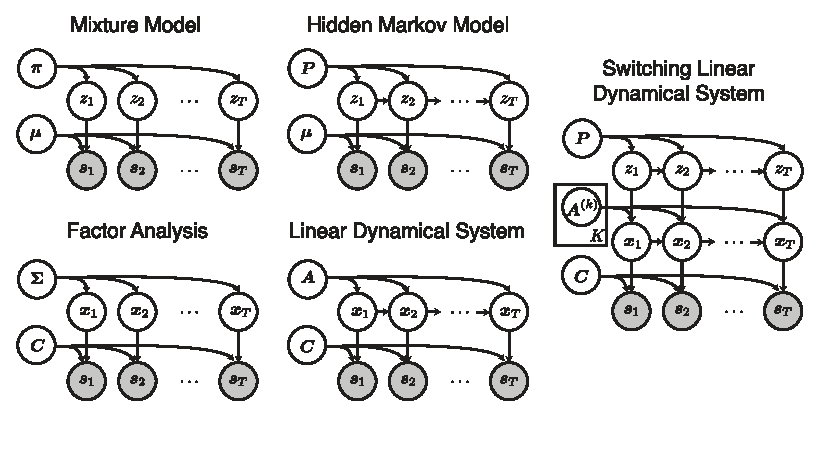
\includegraphics[width=5.5in]{figures/ch8/graphical_models} 
\vspace{-.25in}
\caption{Special cases of the switching linear dynamical system.
  Adapted from Figure~\ref{fig:motifs}.}
\label{fig:slds_models}
\end{figure}

The graphical models corresponding to these special cases are shown in
Figure~\ref{fig:slds_models}, with the omission of some model
parameters to conserve space. This figure is adapted from
Figure~\ref{fig:motifs}. The only model that is not captured here
is the autoregressive model since, here, all interaction between
spike counts arises through the latent state. Next we show how
a single, unified algorithm can support efficient
inference in the SLDS and all its special cases.


\section{Markov chain Monte Carlo Inference}


First we show how the continuous latent states,~$\bx_{1:T}$, can be
updated with a block Gibbs sampler when the spikes are conditionally
Gaussian distributed.  While unrealistic for neural spike trains, the
key elements of the inference algorithm will be conserved when we move
to discrete count observations.  Given the Gaussian inference
algorithm, we will show how the \polyagamma augmentation explored in
Chapter~\ref{chap:five} enables efficient, fully-conjugate Bayesian
inference in discrete models as well.

\subsection{Block Gibbs Sampling Latent States with Gaussian Observations}
Suppose the spike counts,~$\bs_t$ were conditionally distributed
according to a Gaussian distribution. Moreover, assume the
distribution has nonstationary precision,~$\bOmega_t$, such that
\begin{align}
  \label{eq:gauss_lkhd}
  p(\bs_t \given \bx_t, \btheta) 
  &=
  \distNormal(\bs_t \given \bC \bx_t, \bOmega_t^{-1}).
\end{align}
In this case, the conditional distribution over continuous latent
states,~${p(\bx_{1:T} \given \bs_{1:T}, \bz_{1:T}, \btheta)}$, is
jointly Gaussian as well.  The marginal ``filtered'' distribution
given observations up to time~$t$ is a Gaussian, which we will denote
by,
\begin{align*}
  p(\bx_t \given \bs_{1:t}, \bz_{1:t}, \btheta) &= \distNormal(\bx_t \given \bbm_t, \bV_t),
\end{align*}
where~$\bbm_t$ and~$\bV_t$ are the filtered mean and covariance, respectively.

Kalman filtering is an iterative algorithm for computing these filtered means 
and variances. 
Here, we follow the presentation of
\citet[Chapter 18]{murphy2012probabilistic}.  Kalman filtering consists
of iterating forward in time from~${t=1}$ to~${t=T}$. Assume that at iteration~$t$ we
have already computed~$\bbm_{t-1}$ and~$\bV_{t-1}$. Given the
Markovian structure of the probabilistic model, the
conditional distribution of~$\bx_t$ factors into,
\begin{align*}
  p(\bx_t \given \bs_{1:t}, \bz_{1:t}, \btheta)
  &\propto
  \underbrace{p(\bs_t \given \bx_t, \btheta)}_{\text{condition}} \,
  \underbrace{p(\bx_{t} \given \bs_{1:t-1}, \bz_{1:t}, \btheta)}_{\text{predict}}.
\end{align*}
We will show that both of these factors are Gaussian distributions, 
and hence their product is as well. 

%To compute its paramters, we perform two steps: we \emph{predict} its
%value given preceding observations, and then we
%\emph{condition} on the current observation. 

The first step is to \emph{predict}~$\bx_t$ given observations~$\bs_{1:t-1}$.
To do so, we marginalize over the previous latent state,~$\bx_{t-1}$,
\begin{align*}
  p(\bx_t \given \bs_{1:t-1}, \bz_{1:t}, \btheta)
  &\propto  \int p(\bx_t \given \bx_{t-1}, z_{t}, \btheta) \, 
    p(\bx_{t-1} \given \bs_{1:t-1}, \bz_{1:t-1}, \btheta) \, \mathrm{d} \bx_{t-1} \\
  &= \distNormal(\bx_t \given \bbm_{t|t-1}, \bV_{t|t-1}),
\end{align*}
where
\begin{align*}
  \bbm_{t|t-1} &\triangleq \bA_t \bbm_{t-1} + \bb_t \\
  \bV_{t|t-1} &\triangleq \bA_t \bV_{t-1}\bA_t^\trans + \bSigma_t.
\end{align*}
Then, we \emph{condition} on the current observations,~$\bs_t$, to get the
parameters of the filtered distribution,
\begin{align}
  \nonumber
  \bbm_t &= \bbm_{t|t-1} + \bK_t (\bs_t - \bC \bbm_{t|t-1}) \\
  \label{eq:kalman_filter}
  \bV_t &= (\bI - \bK_t \bC) \bV_{t|t-1},
\end{align}
where~$\bK_t$ is the ``Kalman gain'' matrix,
\begin{align*}
  \bK_t &\triangleq \bV_{t|t-1} \bC^\trans \left[ \bC \bV_{t|t-1} \bC^\trans + \bOmega_t^{-1} \right]^{-1}.
\end{align*}

Once we have computed the filtered means and covariances for all
time bins, we can sample from the joint distribution over~$\bx_{1:T}$
by applying the chain rule,
\begin{align*}
  p(\bx_{1:T} \given \bs_{1:T}, \bz_{1:T}, \btheta)
  &= p(\bx_T \given \bs_{1:T}, \bz_{1:T}, \btheta)
  \prod_{t} p(\bx_{t} \given \bx_{t+1:T}, \bs_{1:T}, \bz_{1:T}, \btheta) \\
  &\propto p(\bx_T \given \bs_{1:T}, \bz_{1:T}, \btheta)
  \prod_{t} p(\bx_t \given \bs_{1:t}, \bz_{1:t}, \btheta) \, 
    p(\bx_{t+1} \given \bx_{t}, z_{t+1}, \btheta).
\end{align*}
Thus, we can sample in reverse order, starting with~$\bx_T$ and ending
with~$\bx_1$. The conditional distribution of~${\bx_t}$
\begin{align}
  \label{eq:bkwd_sample}
  p(\bx_t \given \bx_{t+1:T}, \bs_{1:T}, \bz_{1:T}, \btheta)
  &\propto
  \distNormal(\bx_t \given \bbm_t, \bV_t) \,
  \distNormal(\bx_{t+1} \given \bA_{t+1}\bx_{t} + \bb_{t+1}, \bSigma_{t+1}),
\end{align}
which is yet another Gaussian distribution. Now we can write the complete 
algorithm for block Gibbs sampling the continuous latent states,~$\bx_{1:T}$.

\begin{center}
  \begin{minipage}{.75\textwidth}
    \vskip-2em
    \singlespacing
    \begin{algorithm}[H]
      \sffamily
      \begin{algorithmic}
        \Require $\bs_{1:T}$, $\bz_{1:T}$, $\btheta$ 
        \For {$t = 1, \ldots, T$}
          \State Compute~$\bbm_t$ and~$\bV_t$ \Comment{Eq.~\ref{eq:kalman_filter}}
        \EndFor
        \For {$t = T, \ldots, 1$}
          \State Sample~$\bx_t \given \bx_{t+1}, \bbm_t, \bV_t, \btheta$ \Comment{Eq.~\ref{eq:bkwd_sample}}
        \EndFor
      \end{algorithmic}
      \caption{Forward filtering, backward sampling algorithm for the Gaussian linear dynamical system.}
      \label{alg:ffbs_gaussian_lds}
    \end{algorithm}
  \end{minipage}
\end{center}


% The rest of the MCMC algorithm is straightforward. We can perform a
% block Gibbs update for~$\bz_{1:T}$ in much the same way as we did
% for~$\bx_{1:T}$. The HMM message passing algorithms of the last
% chapter are easily extended to handle this case. Finally, sampling the
% parameters, like~$\bA_k$,~$\bb_k$, and~$\bSigma_k$, is straightforward as
% well.  The problem reduces to one of inference in a Bayesian linear
% regression model once we have conditioned on~$\bz$,~$\bx$, and~$\bs$.

\subsection{\polyagamma Augmentation for Discrete Observations}
The conditional distribution of the latent states is only Gaussian
if the observations are as well. Fortunately, we can make the
observations effectively \emph{look} Gaussian by augmenting the
data with \polyagamma auxiliary variables. 
Recall from Chapter~\ref{chap:five} that the \polyagamma augmentation
is an auxiliary variable scheme that applies to models with logistic
link functions \citep{polson2013bayesian}.  This augmentation can be
used to develop Gibbs for models with likelihoods of the form,
\begin{align*}
  \nonumber  p(s \given \psi, \nu)
  &= c(s, \nu) \, \sigma(\psi)^{a(s, \nu)} \,
  (1-\sigma(\psi))^{d(s, \nu)} \\
  &= c(s, \nu)
  \frac{(e^{\psi})^{a(s, \nu)}}
       {(1+e^{\psi})^{b(s, \nu)}}.
\end{align*}
These are called \emph{logistic likelihoods} because the latent
variables are transformed by a logistic
function,~${\sigma(\psi)=e^\psi /(1+e^\psi)}$.  Bernoulli, binomial,
negative binomial, and multinomial likelihoods can all be put in this
form.  For example, in the Bernoulli
case,
\begin{align*}
  \distBernoulli(s \given \psi) 
  &= \sigma(\psi)^{s}
    (1-\sigma(\psi))^{1-s}
  = \frac{(e^{\psi})^{s}}
       {(1+e^{\psi})}.
\end{align*}
Thus,~${a(s, \nu) = s}$,
${b(s,\nu) \equiv 1}$, and~${c(s, \nu) \equiv 1}$.
We refer back to Table~\ref{tab:obs_models} for the formulation of
other count distributions.

The augmentation is based on an integral identity
derived from the Laplace transform of the \polyagamma distribution.
Specifically, if $p_{\distPolyaGamma}(\pgvar\given b, 0)$ is the
density of the \polyagamma distribution,~${\distPolyaGamma(b, 0)}$,
then,
\begin{align}
  \frac{(e^{\psi})^a}{(1+e^{\psi})^b}
  &= 2^{-b} e^{\kappa \psi}
  \int_{0}^{\infty} e^{-\pgvar \psi^2 /2} \,
  p_{\distPolyaGamma}(\pgvar \given b, 0) \, \mathrm{d}\pgvar,
\label{eq:pg_identity_new}
\end{align}
where~${\kappa=a-b/2}$. The integral on the right-hand side is the
Laplace transform of the \polyagamma density evaluated at~$\psi^2/2$,
and the left-hand side is the same form found in discrete
distributions with logistic link functions.  Importantly, viewed as a
function of~$\psi$ for fixed~$\pgvar$, the right-hand side is an
unnormalized Gaussian density.  Thus, the identity
in~\eqref{eq:pg_identity_new} transforms a logistic likelihood to a
Gaussian likelihood conditioned on an auxiliary variable,~$\pgvar$.

Now, let us return to the likelihood of~\eqref{eq:s_likelihood},
where~${\psi_{t,n} = [\bC \bx_t]_n = \bc_n^\trans \bx_t}$ is the activation of neuron $n$
at time~$t$. As a function of~$\bx_t$, the likelihood is proportional to,
\begin{align*}
  p(\bs_t \given \bx_t, \btheta)
  &\propto \prod_{n=1}^N 
  \frac{(e^{\psi_{t,n}})^{a(s_{t,n}, \nu_n)}}
       {(1+e^{\psi_{t,n}})^{b(s_{t,n}, \nu_n)}} \\
  &\propto \prod_{n=1}^N 
     e^{\kappa(s_{t,n}, \nu_n) \psi_{t,n}}
  \int_{0}^{\infty} e^{-\pgvar_{t,n} \psi_{t,n}^2 /2} \,
  p_{\distPolyaGamma}(\pgvar_{t,n} \given b(s_{t,n}, \nu_n), 0) \,
  \mathrm{d}\pgvar_{t,n}.
\end{align*}
If rather than integrating over~$\omega_{t,n}$ explicitly, we instead
augment our data by introducing~$\omega_{t,n}$ as auxiliary variables,
the likelihood of~$\bx_t$ is proportional to a multivariate Gaussian
distribution,
\begin{align}
  \nonumber
  p(\bs_t \given \bx_t, \bomega_t, \{\nu_n\})
  &\propto \prod_{n=1}^N
  \distNormal(\bc_n^\trans \bx_t \given
  \omega_{t,n}^{-1} \kappa(s_{t,n}, \nu_n), \,
  \omega_{t,n}^{-1}) \\
  \label{eq:pg_likelihood}
  &\propto \distNormal(
  \widehat{\bs}_t \given
  \bC \bx_t, \, 
  \bOmega_t^{-1}),
\end{align}
where
\begin{align*}
  \widehat{\bs}_t &= \bOmega_t^{-1} \kappa(\bs_t, \nu_n) \\
  \bOmega_t &= \diag \left( \left[ \omega_{t,1}, \ldots, \omega_{t,N} \right] \right).
\end{align*}
Note the similarity between the augmented likelihood
of~\eqref{eq:pg_likelihood} and the Gaussian likelihood
of~\eqref{eq:gauss_lkhd}. The only difference is that, here, the
precision is given by the auxiliary variables, and the ``effective''
observations,~$\widehat{s}_{t,n}$, are a function of
both~$s_{t,n}$,~$\omega_{t,n}$, and~$\nu_n$.  Thus, given a set of
\polyagamma auxiliary variables, the block Gibbs updates in
Algorithm~\ref{alg:ffbs_gaussian_lds} will apply equally well to the
setting with discrete count observations.

Moreover, by the exponential tilting property of the \polyagamma
distribution, the conditional distribution of~$\pgvar_{t,n}$
is proportional to a \polyagamma distribution:
\begin{align}
  \nonumber
  p(\pgvar_{t,n} \given \psi_{t,n}, s_{t,n}, \nu_n) &
  \propto e^{-\pgvar_{t,n} \psi_{t,n}^2/2} \,
  p_{\distPolyaGamma}(\pgvar_{t,n} \given b(s_{t,n}, \nu_n), \, 0) \\
  \label{eq:omega_conditional}
  &\propto p_{\distPolyaGamma}(\pgvar_{t,n} \given b(s_{t,n}, \nu_n), \, \psi_{t,n}).
\end{align}
These auxiliary variables are conditionally independent of each other,
and hence amenable to block parallel Gibbs sampling.  Efficient
\polyagamma sampling algorithms have been developed for the regimes
typically encountered in Bernoulli, binomial, and negative binomial
models \citep{windle2014sampling}.

%When the shape parameter,~$b(x_n, \nu_n)$, goes to zero, the
%\polyagamma density reduces to a delta function at zero. 
The proposed algorithm for sampling the latent variables and 
parameters of an SLDS is summarized in Program~\ref{alg:slds}.

\begin{center}
  \begin{minipage}{.75\textwidth}
    \vskip-2em
    \singlespacing
    \begin{algorithm}[H]
      \sffamily
      \begin{algorithmic}
        \Require $\bs_{1:T}$ and $\bz_{1:T}$, $\bx_{1:T}$, and $\btheta$ from previous iteration
        \State Sample $\btheta \given \bz_{1:T}, \bx_{1:T}, \bs_{1:T}$
        \State Sample $\bz_{1:T} \given \bx_{1:T}, \btheta$ 
        \Comment{HMM update}
        \For {$t = 1, \ldots, T$} \Comment{In parallel}
          \For {$n = 1, \ldots, N$}  \Comment{In parallel}
            \State Sample $\omega_{t,n} \given s_{t,n}, \bx_t, \btheta$ 
            \Comment{Eq.~\ref{eq:omega_conditional}}
          \EndFor
        \EndFor
        \State Compute $\bOmega_{1:T}$ and~$\widehat{\bs}_{1:T}$ \Comment{Eq.~\ref{eq:pg_likelihood}}
        \State Sample $\bx_{1:T} \given \widehat{\bs}_{1:T}, \bz_{1:T}, \bOmega_{1:T}, \btheta$ 
        \Comment{Algorithm~\ref{alg:ffbs_gaussian_lds}}
      \end{algorithmic}
      \caption{Single iteration of Gibbs sampler for an switching LDS with discrete count observations}
      \label{alg:slds}
    \end{algorithm}
  \end{minipage}
\end{center}


\subsection{Missing Data}
Sometimes we only have partial observations. For example, in some cases we have 
multiple recordings from the same circuit, but each recording only provides access 
to a subset of the population of neurons \citep{turaga2013inferring}. In other cases,
we simply hold out some of the data for predictive likelihood comparisons. With
Gaussian observations, we can implement this by replacing the missing data point,~$s_{t,n}$,
with a zero mean, zero precision observation. In the discrete count model, this can 
be implemented by setting the auxiliary variable,~$\omega_{t,n}$, to zero. Recall 
that the \polyagamma auxiliary variables specify the precision of the effective 
observations. By setting this to zero, and also setting the mean~$\kappa(s_{t,n}, \nu_n)$
to zero, we can effectively remove this data point. 
%In the experiments below, we will use this approach
%to withhold a subset of spike counts during training.

\section{Alternative approaches}
Most alternative approaches to performing Bayesian inference in latent
state space models with discrete observations have relied on a Laplace
approximation \citep{tierney1986accurate} to the conditional
distribution,~${p(\bx_{1:T} \given \bs_{1:T}, \bz_{1:T}, \btheta)}$
\citep{Smith-2003, paninski2010new, macke2011empirical}
\footnote{While the Laplace approximation is most common, see 
  \citet{buesing2012spectral} and \citet{pfau2013robust} for some
  interesting new directions.}. Given a
Gaussian approximation, the model parameters,~$\btheta$, can be
optimized such that they maximize the \emph{expected} joint log
probability under the approximate Gaussian distribution on~$\bx$. This
constitutes an approximate expectation-maximization (EM) algorithm
\citep{dempster1977maximum}.

\sloppy
For completeness, we describe the fundamentals of this approach,
largely following the presentation of~\citet{macke2011empirical}.
Consider a generative model in which~${s_{t,n} \sim \distPoisson(\exp\{\bc_n^\trans \bx_t\})}$.  The conditional log probability of~$\bx_{1:T}$ is
given by,
\begin{align*}
  \log p(\bx_{1:T} \given \bs_{1:T}, \bz_{1:T}, \btheta)
  &\simeq \sum_{t=1}^T \sum_{n=1}^N s_{t,n} (\bc_{n}^\trans \bx_{t}) - \exp\{\bc_n^\trans\bx_{t}\} + \\
  &-\frac{1}{2} (\bx_1 - \bmu_1)^\trans \bSigma_{z_1}^{-1} (\bx_1 - \bmu_1) + \\
  &-\frac{1}{2} \sum_{t=2}^T (\bx_t - \bA_{z_t} \bx_{t-1} - \bb_{z_t})^\trans
  \bSigma_{z_t}^{-1} (\bx_t - \bA_{z_t} \bx_{t-1} - \bb_{z_t}),
\end{align*}
where~$\simeq$ denotes equality up to an additive constant.
This log probability is concave and can be efficiently maximized to
obtain the mean of the Laplace approximation,
\begin{align*}
  \bmu^* &= \argmax_{\bx_{1:T}}
  \log p(\bx_{1:T} \given \bs_{1:T}, \bz_{1:T}, \btheta).
\end{align*}
Once the mean has been found, the optimal covariance is given by
the inverse Hessian of the log posterior evalulated at~$\bmu^*$,
\begin{align*}
  \bSigma^* &= - \left[ \nabla \nabla_{\bx_{1:T}}
      \log p(\bx_{1:T} \given \bs_{1:T}, \bz_{1:T}, \btheta) \, \Big|_{\bx_{1:T}=\bmu^*} \right]^{-1}.
\end{align*}
By exploiting the chain structure of the graphical model, this
inverse Hessian can be computed in time linear in~$T$ using essentially
the same forward-backward approaches used during sampling.

The mean and covariance parameterize a Gaussian approximation,
\begin{align*}
  p(\bx_{1:T} \given \bs_{1:T}, \bz_{1:T}, \btheta)
  &\approx
  q(\bx_{1:T}) =
  \distNormal(\bx_{1:T} \given \bmu^*, \bSigma*).
\end{align*}
Given this approximation, the parameters are updated by maximizing
the expected log probability,
\begin{align*}
  \btheta^*
  &=
  \argmax_{\btheta} \bbE_{q} \left[ \log p(\bs_{1:T}, \bx_{1:T}, \bz_{1:T}, \btheta) \right]. 
\end{align*}
For example, consider this expectation as a function of the emission
matrix,~$\bC$,
\begin{align*}
  \bbE_q \left[ \log p(\bs_{1:T}, \bx_{1:T}, \bz_{1:T}, \btheta) \right]
  &\simeq
  \sum_{t=1}^T \sum_{n=1}^N s_{t,n} (\bc_{n}^\trans \bbE_q[\bx_{t}]) - \bbE_q\left[\exp\{\bc_n^\trans \bx_{t}\} \right], \\
  &=
  \sum_{t=1}^T \sum_{n=1}^N s_{t,n} (\bc_{n}^\trans \bmu_{t}^*)
  - \exp \left\{
  \bc_n^\trans \bmu_t^*  +\frac{1}{2} \bc_n^\trans \bSigma_{tt}^* \bc_n
  \right\}.
\end{align*}
The last line follows from the moment generating function of the
multivariate Gaussian distribution.  This objective function is
concave in~$\bc_n$. Note that closed form, concave expectations
arise from the particular choice of exponential link function.
Other models may require Monte Carlo estimates of the expectation
inside the optimization. As more and more approximation is required,
the performance of these methods tends to suffer.

Finally, we must handle the discrete latent states,~$\bz_{1:T}$.
The simplest approach would be to alternate between updating the
discrete and continuous latent states, as we have advocated in the
MCMC algorithm presented above. Alternatively, \citet{Petreska-2011}
have suggested a joint update for both~$\bx_{1:T}$ and~$\bz_{1:T}$
based on an approximate filtering technique. We leave a detailed
comparison of these two approaches to future work.

From our perspective, the principal advangages of the \polyagamma
augmentation are: (i) it allows for simple block Gibbs updates that
leverage off-the-shelf code for Gaussian models; (ii) it provides an
asymptotically unbiased estimate of the posterior distribution;
(iii) the stochasticity of the MCMC transitions allows the sampling
algorithm to escape local modes, to which expectation-maximization
algorithms are prone \citep{bishop2006pattern}; and (iv) once we
have an MCMC algorithm, a number of natural extensions are clear,
like the marginal likelihood estimation methods we discuss next.

\section{Model Comparison via Marginal Likelihood Estimation}
The marginal likelihood of a model is the probability of the
data,~$\bs$, having integrated out the latent
variables,~$\bz$ and~$\bx$, and the parameters,~$\btheta$,
\begin{align*}
  p(\bs) = \int p(\bs \given \bz, \bx, \btheta) \, 
  p(\bz, \bx, \btheta) \, \mathrm{d} \bz \, \mathrm{d}\bx \, \mathrm{d}\btheta
\end{align*}
By integrating over the latent variables and parameters, the marginal
likelihood captures a tradeoff between a model's complexity and its
ability to explain the data.  As such, it is a natural criterion for
model comparison. For conjugate exponential family 
models, like linear Gaussian models with Gaussian observations,
 the marginal likelihood can be computed in closed form. 
In these cases, marginal likelihood is often the gold-standard 
for model selection \citep{kass1995bayes}.

Unfortunately, minor adjustments to the model can render the
integration over parameters and latent variables intractable.  For
example, the marginal likelihood is intractable the SLDS models 
with discrete observations we have just described. 
Instead, we are forced to resort to approximate methods like annealed
importance sampling (AIS) \citep{neal2001annealed}.  AIS is based on
sampling from a sequence of intermediate distributions that
\emph{anneal} between a tractable distribution and the intractable
posterior. While AIS has proven highly effective for a variety of
models \citep{grosse2015sandwiching}, the accuracy of the method hinges
upon the efficiency of the Markov transition operators that target
the intermediate distributions.  Unfortunately, these distributions
often lack exploitable structure present in the posterior, making the
design of efficient transition operators challenging, and ultimately
compromising the efficacy of AIS. We will show how the \polyagamma 
augmentation strategies above can be extended to perform efficient 
annealed importance sampling in the class of switching linear dynamical
 systems models with count observations.

\subsection{Annealed Importance Sampling}

\sloppy
Annealed importance sampling \citep{neal2001annealed} is a method of
estimating the marginal likelihood,~$p(\bs)$, by ``annealing'' between
a tractable distribution, with known normalization constant, and the
joint distribution, whose normalization constant is the marginal
likelihood of interest. The annealing path is a sequence of
distributions,~${q_1(\btheta, \bz, \bx)}$ to~${q_M(\btheta, \bz, \bx) = p(\btheta, \bz, \bx \given \bs)}$,
where
\begin{align*}
q_m(\btheta, \bz, \bx) &= \frac{f_m(\btheta, \bz, \bx)}{\mcZ_m}, & 
f_M(\btheta, \bz, \bx) &= p(\theta, \bz, \bx, \bs), & 
\mcZ_M &= p(\bs).
\end{align*}
Typically, we let~$q_1(\btheta, \bz, \bx)$ be the normalized prior
distribution such
that~${f_1(\btheta, \bz, \bx) = p(\btheta, \bz, \bx)}$
and~${\mcZ_1=1}$. Then, we let~$f_m(\bz, \theta)$ be a geometric
average of the prior and the joint:
\begin{align*}
  f_m(\btheta, \bz, \bx) 
  &=
  \Big[ p(\btheta, \bz, \bx) \Big]^{1-\beta_m} \,
  \Big[ p(\btheta, \bz, \bx, \bs) \Big]^{\beta_m} \\
  &= p(\btheta, \bz, \bx) \, p(\bs \given \btheta, \bz, \bx)^{\beta_m},
\end{align*}
with~$\beta_m$ monotonically increasing from~${\beta_1=0}$ to~${\beta_M=1}$.
As we anneal between~$0$ and~$1$, the intermediate distributions 
interpolate between the prior and the unnormalized posterior.

Given this annealing path, we can generate a sample
of~$(\btheta, \bz, \bx)$ by first sampling from the prior, and then
applying a sequence of MCMC transition operators that leave
the intermediate distributions~$q_m$ invariant,
\begin{align*}
  \mcT_m(\btheta, \bz, \bx \from \btheta', \bz', \bx').
\end{align*}
The result of applying these transition operators
for~${m=1, \ldots, M}$ is a sample that is, hopefully, closer in
distribution to the posterior. We can use this procedure as a proposal
distribution for importance sampling.  The importance weights are
given by a product of ratios between~$f_m$ and~$f_{m-1}$.  Since the
target density is the unnormalized joint distribution, the importance
weights will be unbiased estimates of the normalization constant,
namely the marginal likelihood,~${\mcZ_M =p(\bs)}$. The annealed
importance sampling algorithm is summarized in Algorithm~\ref{alg:ais}.
\begin{center}
  \begin{minipage}{.85\textwidth}
    \vskip-2em
    \singlespacing
    \begin{algorithm}[H]
      \sffamily
      \begin{algorithmic}
        %\Require $\bs_{1:T}$
        \For {$\ell=1$ to~$L$}
          \State $w^{(k)} \from \mcZ_1$
          \State Sample $\btheta^{(1)}, \bz^{(1)}, \bx^{(1)} \sim q_1(\btheta, \bz, \bx)$
          \For {$m=2$ to~$M$}
            \State 
            ${
              w^{(\ell)} \from w^{(\ell)} \times 
              \frac{f_m(\btheta^{(m-1)}, \,  \bz^{(m-1)}, \, \bx^{(m-1)})}
              {f_{m-1}(\btheta^{(m-1)}, \, \bz^{(m-1)}, \, \bx^{(m-1)})}
            }$
            \State Sample ${\btheta^{(m)}, \bz^{(m)}, \bx^{(m)} \sim 
              \mcT_m (\btheta, \bz, \bx \from \btheta^{(m-1)}, \,  \bz^{(m-1)}, \, \bx^{(m-1)})}$
          \EndFor
        \EndFor\\
        \Return {$\widehat{\mcZ}_M = \frac{1}{L} \sum_{\ell=1}^L w^{(\ell)} $}
      \end{algorithmic}
      \caption{Annealed Importance Sampling (AIS). Adapted from \citep{grosse2015sandwiching}.}
      \label{alg:ais}
    \end{algorithm}
    \vspace{.5em}
  \end{minipage}
\end{center}

How can we reduce the variance of this estimator? First, we can
increase the number of intermediate distributions; second, we can
design rapidly mixing transition operators,~$\mcT_m$. In this section,
we develop transition operators that are both computationally efficient,
allowing us to run more transitions in a fixed amount of time, and more
effective, in that they quickly reach their equilibrium distribution.

With a geometric annealing path, the intermediate distributions of the 
switching LDS are given by,
\begin{align}
  \label{eq:intermediate}
  f_m(\btheta, \bz, \bx) 
  &= p(\btheta, \bz, \bx) \,  
    \prod_{t=1}^T \prod_{n=1}^N
    c(s_{t,n}, \btheta)^{\beta_m} \frac{(e^{\psi_{t,n}})^{a(s_{t,n}, \btheta) \cdot \beta_m}}
    {(1+e^{\psi_{t,n}})^{b(s_{t,n}, \btheta) \cdot \beta_m}}.
\end{align}
where, again,~$\psi_{t,n}$ is a function of~$\bx$ and~$\btheta$.
Raising the likelihood to the power~$\beta_m$ does change its
functional form; it only changes the power in the exponent.
Most importantly, it is still amenable to \polyagamma augmentation!
Thus, the Gibbs sweep defined in Algorithm~\ref{alg:slds} can be used as
a transition operator,~$\mcT_m$.

However, for this transition to be efficient, we must be able to
sample from the \polyagamma conditional distribution in the regime
where~${b(s_{t,n}, \btheta) \cdot \beta_m < 1}$.  For Bernoulli
observations,~${b(s_{t,n}, \btheta) \equiv 1}$, so we will be in this
regime for all~$\beta_m \in [0,1)$.  While efficient samplers exist
for \polyagamma distributed variables when the shape parameter is
greater than or equal to one \citep{windle2014sampling}, this ``small shape''
regime has not been previously explored.  We develop a novel sampling
algorithm that makes these conditional updates extremely efficient,
and renders AIS with \polyagamma augmented transitions highly
effective.

\section{A Novel Sampling Algorithm for the \polyagamma Distribution}
\label{sec:pgsampling}

The \polyagamma distribution,~$\distPolyaGamma(b,\psi)$, is closely related 
to the Jacobi distribution,~$\distJacobi(b,\psi)$, surveyed by \citet{biane2001probability} and 
elaborated upon in~\citet{windle2014sampling}.
Specifically, 
\begin{align*}
  \distPolyaGamma(b, \psi) \sim \frac{1}{4} \distJacobi(b, \tfrac{\psi}{2}).
\end{align*}
Thus, to develop a sampler for the \polyagamma distribution, 
it is sufficient to be able to sample the Jacobi distribution.

As derived by \citet{windle2014sampling}, the density
of~$\distJacobi(b,\psi)$ can be written as an infinite alternating
sum,
\begin{multline}
  \label{eq:jacobi_density}
  p_{\distJacobi}(\pgvar \given b, \psi) = \\ 
  \cosh^b(\psi) e^{-\pgvar \psi^2/2} \frac{2^b}{\Gamma(b)} 
  \sum_{n=0}^\infty (-1)^n \frac{\Gamma(n+b)}{\Gamma(n+1)} \frac{(2n+b)}{\sqrt{2\pi \pgvar^3}}
  \exp\left\{- \frac{(2n+b)^2}{2\pgvar} \right\}.
\end{multline}
\citet{windle2014sampling} developed a number of methods for sampling
this distribution. Most rely on finding tractable upper bounds on the density
that can serve as a proposal distribution. Given a sample from the proposal,
it is possible to accept or reject using the \emph{alternating series method} \citep{devroye1986}. We will go into more detail on this shortly.

We take the same basic approach, but we present a novel means of
finding an upper bound on the Jacobi density.  Massaging terms
in~\eqref{eq:jacobi_density}, we can factor this into the product of
three terms:
\begin{align*}
  % \nonumber &p_{\distJacobi}(\pgvar \given b, \psi) \\
  % \nonumber &\quad= \cosh^b(\psi) \frac{b 2^b}{\sqrt{2\pi \pgvar^3}} 
  %   \exp \left \{ -\frac{b^2}{2\pgvar} - \frac{\pgvar \psi^2}{2} \right \}
  %   \Phi(\pgvar \given b) \\
  % &= \cosh^b(\psi) \frac{b 2^b}{\sqrt{2\pi \pgvar^3}} 
  %   \exp \left \{ -\frac{\psi^2}{2\pgvar} \left[\left( \frac{b}{\psi} \right)^2 + \pgvar^2 \right]\right \}
  %   \left( 1-\Phi(\pgvar \given b) \right) \\
  % &= \cosh^b(\psi) \frac{b 2^b}{\sqrt{2\pi \pgvar^3}} 
  %   \exp \left \{ -\frac{\psi^2}{2\pgvar} \left[\left( \pgvar- \frac{b}{|\psi|} \right)^2  +\frac{2b\pgvar}{|\psi|}\right]\right \}
  %   \left( 1-\Phi(\pgvar \given b) \right) \\
  %&= \cosh^b(\psi) \frac{b 2^b}{\sqrt{2\pi \pgvar^3}} 
  %  \exp \left \{ -\frac{\left(\tfrac{|\psi|}{b}\right)^2 b^2}{2\pgvar} \left( \pgvar- \frac{b}{|\psi|} \right)^2  
  %  -b|\psi| \right \} 
  %  \left( 1-\Phi(\pgvar \given b) \right) \\
  % &\quad = 2^b \, \cosh^b(\psi) \, e^{-b|\psi|} \,
  %   p_{\distInvGaussian} \left(\pgvar \, \bigg| \, \frac{b}{|\psi|}, \, b^2 \right) 
  %   \Phi(\pgvar \given b),
  p_{\distJacobi}(\pgvar \given b,\psi) &= 
   \alpha^{-1}(b,\psi) \,
   p_{\distInvGaussian}\left(\pgvar \, \bigg| \, \frac{b}{|\psi|}, \, b^2 \right) \,
   \Phi(\pgvar \given b).
\end{align*}
The first term,~$\alpha^{-1}(b,\psi)$, is a scaling constant greater than one,
\begin{align*}
  \alpha^{-1}(b,\psi) = 2^b \, \cosh^b(\psi) \, e^{-b|\psi|} 
  % &= 2^b \cosh^b(|\psi|) \, e^{-b|\psi|} \\
  % &= 2^b \left(\frac{(1+e^{-2|\psi|}) e^{-|\psi|}}{2e^{-|\psi|}} \right)^b \\
  = \left(1 + e^{-2|\psi|} \right)^b \geq 1.
\end{align*}
The second is an inverse Gaussian density,
\begin{align*}
p_{\distInvGaussian} \left(\pgvar \, \bigg| \, \frac{b}{|\psi|}, \, b^2 \right) 
  % &= \left( \frac{b^2}{2\pi \pgvar^3} \right)^{1/2} 
  %   \exp \left \{ - \frac{b^2 \left(\pgvar - \tfrac{b}{|\psi|} \right)^2}{2 \left(\tfrac{b}{|\psi|} \right)^2 \pgvar}   \right \} \\
  &= \frac{b}{\sqrt{2\pi \pgvar^3}}
    \exp \left \{ - \frac{\psi^2}{2\pgvar}  \left(\pgvar - \frac{b}{|\psi|} \right)^2   \right \}.
\end{align*}
And finally, the third term we have called~$\Phi(\pgvar \given b)$, 
\begin{align*}
  \Phi(\pgvar \given b)  
  &= \sum_{n=0}^\infty (-1)^n \frac{\Gamma(n+b)}{\Gamma(n+1)} \frac{2n+b}{\Gamma(b+1)}
    \exp\left\{- \frac{2n(n+b)}{\pgvar} \right\}.  
\end{align*}


\begin{figure}
\centering
  \begin{subfigure}[t]{2.7in}
    \caption{}
    \label{fig:pg_phi}
    \vspace{-1em}
    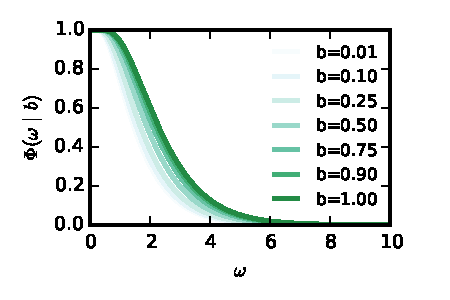
\includegraphics[width=\textwidth]{figures/ch8/phi}
  \end{subfigure}
  \begin{subfigure}[t]{2.7in}
    \caption{}
    \label{fig:pg_acceptance}
    \vspace{-1em}
    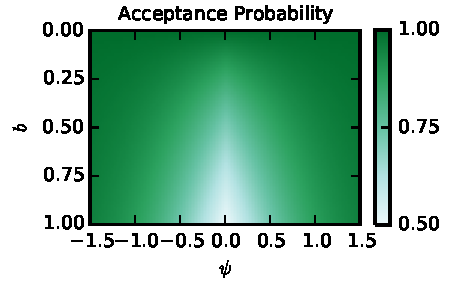
\includegraphics[width=\textwidth]{figures/ch8/acceptance}
  \end{subfigure}
  \vspace{-1em}
  \caption[Rejection sampling algorithm for the \polyagamma
    distribution] {\textbf{(a)} Plot of~$\Phi(\pgvar \given b)$, the
    conditional acceptance probability for a proposed value
    of~$\pgvar$, for a range of~$b\in (0,1]$. In all cases, this function is
  monotonically decreasing from 1 to 0 as a function of~$\pgvar$, and
  thus defines a cumulative distribution function. 
  \textbf{(b)}
  Acceptance probability,~$\alpha(b,\psi)$, as a function of~$b$
  and~$\psi$.}
\label{fig:pgsampling}
\end{figure}

Figure~\ref{fig:pg_phi} plots~$\Phi(\pgvar \given b)$ for various values of~$b$.
In all cases, we see that~$\Phi(\pgvar \given b)$ is a monotonically
decreasing function with,
\begin{align*}
  \lim_{\omega \to 0} \Phi(\omega \given b) &= 1, \\
  \text{and, }
  \lim_{\omega \to \infty} \Phi(\omega \given b) &= 0.
\end{align*}
% , and shows that it is bounded to the range~$[0,1]$.
Since all three terms are non-negative, and since~${\Phi(\pgvar \given
  b) \leq 1}$, the product~${\alpha^{-1}(b,\psi)\,
  p_{\distInvGaussian}(\pgvar \given \tfrac{b}{|\psi|}, b^2)}$
must dominate~$p_{\distJacobi}(\pgvar \given b,\psi)$.  Thus, the inverse
Gaussian is a natural proposal distribution for a rejection sampling
algorithm.  To determine whether a proposed value of~$\pgvar$ is
accepted, we must sample~${u \sim \mathrm{Unif}(0,1)}$, and check
whether~$u < \Phi(\pgvar \given b)$.

The acceptance probability is~$\alpha(b,\psi)$, the inverse of the
scaling constant. It is bounded between~$[\tfrac{1}{2}, 1]$ when~${b
  \leq 1}$.  The lower bound (worst case) is achieved when~${\psi=0}$
and~${b=1}$.  The upper bound (best case) is approached as~$b$ goes to
zero or~$|\psi|$ goes to infinity.  This is illustrated in
Figure~\ref{fig:pg_acceptance} for a range of~$b$ and~$\psi$.
In fact, this rejection sampling algorithm works for~$b \geq 1$ as well,
but as~$b$ increases, the acceptance probability goes to zero. For
this regime, the existing approaches of~\citet{windle2014sampling} are
a better choice.

\paragraph{Determining acceptance}
In order to determine whether to accept or reject a proposed value
of~$\omega$, we need to compare against~${\Phi(\pgvar \given b)}$, for
given~$\pgvar$ and~$b$. This function is not analytically tractable,
however, it is still possible to determine whether or not to accept
with finite computation. To do so, we use a slight modification of the
alternating series method \citep{devroye1986}.  We exploit the
fact that ~$\Phi(\pgvar \given b)$ is an alternating sum, and the
absolute value of the terms is eventually monotonically decreasing as
a function of the index~$n$ for all fixed values of~$b$ an~$\psi$.
Thus, after we have computed the increasing terms, all subsequent
partial sums for even~$n$ are upper bounds, and all subsequent partial
sums for odd~$n$ are lower bounds on~$\Phi(\pgvar\given b)$.  To
determine acceptance of~$u$, we evaluate until we find an upper bound
less than~$u$, at which point we reject, or a lower bound greater
than~$u$, at which point we accept. Empirically, this rarely takes
more than six iterations.

\section{Conclusion}
This chapter has explored various facets of modeling neural spike
trains with switching linear dynamical systems models. This powerful
model for nonlinear dynamical systems contains a number of simpler
models as special cases. We have shown how a simple MCMC inference
algorithm based on the \polyagamma augmentation provides a unified
means of performing inference for the SLDS and its special cases.

As we consider hierarchical models like these --- models constructed out of
layers of latent structure --- we turned our attention to the
important question of model selection. How should we justify our
modeling choices? Marginal likelihood estimates provide one answer
to this question. We have shown how the same \polyagamma augmentations
translate can be applied inside annealed importance sampling algorithms,
one of the most successful means of approximating marginal likelihoods.
In order to make these methods work in practice, however, we needed to
improve the efficiency of sampling the \polyagamma distribution in the
``small shape'' regime. By leveraging a particular decomposition of the
related Jacobi density, we derived an efficient rejection sampling algorithm.

In future work, we will put these novel methods to the test on a variety
of real world modeling problems. For now, however, we turn our attention
to another important question. For all their structure, what can these
models teach us about neural computation. The next chapter provides some
initial attempts to connect the methods we have developed thus far to more
abstract theoretical models of neural computation. 

%%% Commenting out Cosyne experiment results
\begin{comment}
\section{Results}

\begin{figure}
\centering
% Top row: \psi's
  \begin{subfigure}[t]{.26\textwidth}
    \centering
    \vskip 0pt
    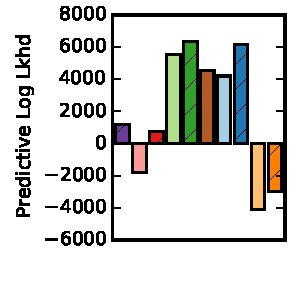
\includegraphics[height=1.4in]{figures/ch8/pred_ll_best_bar.pdf}
    \label{fig:pred_ll_best}
  \end{subfigure}
  ~
  \hspace{-2em}
  \begin{subfigure}[t]{.46\textwidth}
    \centering
    \vskip 0pt
    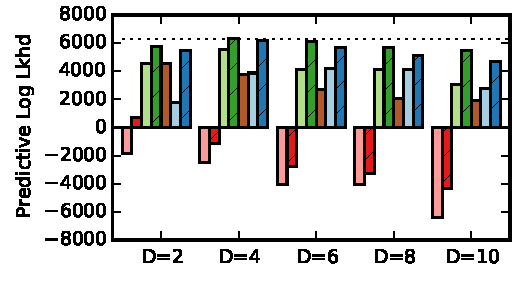
\includegraphics[height=1.4in]{figures/ch8/pred_ll_vs_D_bar.pdf}
  \end{subfigure}
  ~
  \begin{subfigure}[t]{.26\textwidth}
    \centering
    \vskip 0pt
    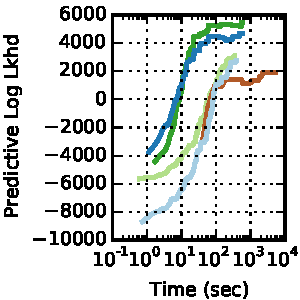
\includegraphics[height=1.4in]{figures/ch8/pred_ll_best_vs_time_D10.pdf}
  \end{subfigure}
  \\
  \begin{subfigure}[t]{\textwidth}
    \centering
    \vskip 0pt
    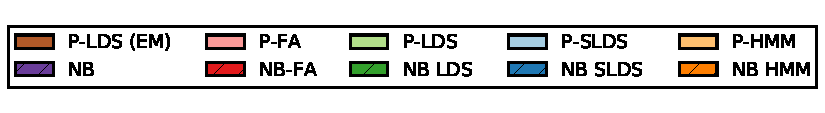
\includegraphics[width=3.8in]{figures/ch8/pred_ll_legend.pdf}
  \end{subfigure}
  \vspace{-1em}
  \caption[Comparison of state space models on hippocampal data]
  {A comparison of latent state space models (FA, LDS, SLDS,
    and HMM) with either Poisson (P) or negative binomial (NB)
    observations fit by our P\'{o}lya-gamma augmented Gibbs sampler to
    a population recording of hippocampal place cells. We measure
    predictive log likelihood on a heldout subset of spike counts and
    find that negative binomial dynamical systems provide the best
    account (left). The latent state space dimensionality,~$D$, is fit
    by cross validation (center), and as the dimension increases the
    models over-fit the training data. Finally, we compare to a
    Poisson LDS (PLDS) model fit via EM and find that our algorithms
    are comparably fast, especially when~$D$ is large
    (right,~$D=10$).}
  \label{fig:hipp8}
\end{figure}


First, we studied a population of 47 hippocampal place cells recorded from a freely moving rat in a 
circular arena.\footnote{Data courtesy of the Wilson lab at MIT.} Spikes were counted in 
250ms bins for approximately ten minutes.
 We held out half of the spike counts (randomly sampled) to compute the predictive 
likelihood of each model relative to a constant-rate Poisson model baseline. 
Figure~\ref{fig:hipp8} shows the results of our comparison for a negative binomial model with constant 
activation and FA, HMM's, LDS's, and switching LDS's with both Poisson and negative binomial observations,
all fit using our augmented MCMC inference algorithm.  We found that the simple FA models over-fit the 
training data and performed poorly on generalization tasks. HMMs, which 
have no low dimensional continuous latent state to tether neurons together, 
performed even worse on predictive tasks. By contrast, the LDS and SLDS 
models and SLDS models exploited temporal dynamics in order to inform latent state estimates.
We explored the effect of the latent state space dimensionality (center panel) and found that 
the LDS and SLDS models generalized well with 4 to 6 dimensional latent states. 
In all cases, the negative binomial 
observation models provided a better fit to the data, suggesting that these 
spike counts were indeed overdispersed (i.e. had variance larger than the mean). With 
our framework, fitting a negative binomial model requires simply changing the 
coefficients of the observation model.

We also compared to a Poisson LDS fit via EM, following \citep{macke2011empirical},
and found that predictive log likelihood estimates with state sequences drawn from 
their variational posterior yield poor predictive estimates. For this dataset, samples 
from our true, non-Gaussian posterior yield more accurate results. Contrary 
to common beliefs about MCMC, our inference algorithms are able to 
explore the posterior parameter space with block Gibbs updates and achieve performance 
that is comparable to EM algorithms, which must solve a large convex optimization problem 
at each iteration (right panel).

Our Bayesian treatment of latent state space models provides a unified 
framework for composing and comparing models of neural activity, and 
identifying latent structure underlying spike trains. As shown with
hippocampal recordings, adopting such an approach allows us to find
a parsimonious description of the neural activity quickly and efficiently
in models that traditionally pose significant inferential challenges.

\end{comment}

